\documentclass{article}
%\usepackage[utf8]{inputenc}
%\usepackage[T1,T2A]{fontenc}
\usepackage[english]{babel}
%\usepackage{amsmath}
%\usepackage{amssymb}
%\usepackage{tikz}
\usepackage{enumitem}
\usepackage{graphicx}
\usepackage{multicol}

\usepackage{wrapfig}
\graphicspath{ {./pic/} }

\usepackage{hyperref}
% \hypersetup{
%     colorlinks=true,
%     linkcolor=black,
%     filecolor=magenta,      
%     urlcolor=cyan,
% }

% black text on white background
\usepackage{xcolor}
\usepackage{pagecolor}
\usepackage{mdframed}
\pagecolor{white}
\color{black}

% better font
\usepackage[defaultsans]{droidsans}
\renewcommand{\sfdefault}{ptm}


\usepackage[a4paper]{geometry}
\usepackage{filecontents, pgffor}

\usepackage[backend=biber]{biblatex}
\addbibresource{Mendeley.bib}
\usepackage{csquotes}

% Copyright 2017 Sergei Tikhomirov, MIT License
% https://github.com/s-tikhomirov/solidity-latex-highlighting/

\usepackage{listings, xcolor}

\definecolor{verylightgray}{rgb}{.97,.97,.97}

\lstdefinelanguage{Solidity}{
	keywords=[1]{anonymous, assembly, assert, balance, break, call, callcode, case, catch, class, constant, continue, contract, debugger, default, delegatecall, delete, do, else, event, export, external, false, finally, for, function, gas, if, implements, import, in, indexed, instanceof, interface, internal, is, length, library, log0, log1, log2, log3, log4, memory, modifier, new, payable, pragma, private, protected, public, pure, push, require, return, returns, revert, selfdestruct, send, storage, struct, suicide, super, switch, then, this, throw, transfer, true, try, typeof, using, value, view, while, with, addmod, ecrecover, keccak256, mulmod, ripemd160, sha256, sha3}, % generic keywords including crypto operations
	keywordstyle=[1]\color{blue}\bfseries,
	keywords=[2]{address, bool, byte, bytes, bytes1, bytes2, bytes3, bytes4, bytes5, bytes6, bytes7, bytes8, bytes9, bytes10, bytes11, bytes12, bytes13, bytes14, bytes15, bytes16, bytes17, bytes18, bytes19, bytes20, bytes21, bytes22, bytes23, bytes24, bytes25, bytes26, bytes27, bytes28, bytes29, bytes30, bytes31, bytes32, enum, int, int8, int16, int24, int32, int40, int48, int56, int64, int72, int80, int88, int96, int104, int112, int120, int128, int136, int144, int152, int160, int168, int176, int184, int192, int200, int208, int216, int224, int232, int240, int248, int256, mapping, string, uint, uint8, uint16, uint24, uint32, uint40, uint48, uint56, uint64, uint72, uint80, uint88, uint96, uint104, uint112, uint120, uint128, uint136, uint144, uint152, uint160, uint168, uint176, uint184, uint192, uint200, uint208, uint216, uint224, uint232, uint240, uint248, uint256, var, void, ether, finney, szabo, wei, days, hours, minutes, seconds, weeks, years},	% types; money and time units
	keywordstyle=[2]\color{teal}\bfseries,
	keywords=[3]{block, blockhash, coinbase, difficulty, gaslimit, number, timestamp, msg, data, gas, sender, sig, value, now, tx, gasprice, origin},	% environment variables
	keywordstyle=[3]\color{violet}\bfseries,
	identifierstyle=\color{black},
	sensitive=false,
	comment=[l]{//},
	morecomment=[s]{/*}{*/},
	commentstyle=\color{gray}\ttfamily,
	stringstyle=\color{red}\ttfamily,
	morestring=[b]',
	morestring=[b]"
}

\lstset{
	language=Solidity,
	backgroundcolor=\color{verylightgray},
	extendedchars=true,
	basicstyle=\footnotesize\ttfamily,
	showstringspaces=false,
	showspaces=false,
	numbers=left,
	numberstyle=\footnotesize,
	numbersep=9pt,
	tabsize=2,
	breaklines=true,
	showtabs=false,
	captionpos=b
}

% Python style for highlighting
\newcommand\pythonstyle{\lstset{
    language=Python,
    basicstyle=\ttm,
    otherkeywords={self},             % Add keywords here
    keywordstyle=\ttb\color{deepblue},
    emph={MyClass,__init__},          % Custom highlighting
    emphstyle=\ttb\color{deepred},    % Custom highlighting style
    stringstyle=\color{deepgreen},
    frame=tb,                         % Any extra options here
    showstringspaces=false            % 
}}


% Python environment
\lstnewenvironment{python}[1][]
{
    \pythonstyle
    \lstset{#1}
}
{}
	% copy the file from this repo

%\selectlanguage{english}

\title{Robonomics: platform for integration of cyber physical systems into human economy \\ \small
\textit{For engineers, smart cities' and Industry 4.0 creators}}
\date{\today}

\author{Sergey Lonshakov \\ Aleksandr Krupenkin \\ Aleksandr Kapitonov, PhD \\ email \href{mailto:research@aira.life}{research@aira.life} \and Evgeny Radchenko \\ Alisher Khassanov \\ Aleksandr Starostin \\ email \href{mailto:engineering@aira.life}{engineering@aira.life} }

\begin{document}
\maketitle
 
\begin{abstract}
Full-scale appliance of cyber physical systems (CPSs) in production, logistics and urban life will allow us to cope with the increasing complexity of supply chains, and deliver quality products to consumers. The main issue here, according to the article's authors, is arranging the global collaboration of different CPSs.

We consider arranging the collaboration of autonomous cyber physical systems' work as a network based on market mechanisms to be the most sustainable option.

The network of distribution, control and provision of services by cyber-physical systems adaptable to human needs, built on the basis of market mechanisms and directly accessible to the end user, can be created on the basis of p2p technologies. This allows the combination of technical and economic parameters of the transaction to the machine.

Building such a peer-to-peer network can be carried out on the basis of the Ethereum infrastructure. By expanding the capabilities of the basic communication protocol, we can train cyber physical systems to interact with market mechanisms and contractual obligations.

The creation and development of a platform that provides tools for working with the robot economy network (briefly - the Robonomics platform) will allow designers of new cities and industrial zones to build trust among the autonomous robots' services, provide direct user access for ordering products from autonomous factories and services of urban sensor networks. This in turn will allow us to put in place a decentralized system that globally monitors the activities of cyber physical systems.
\end{abstract}

\tableofcontents

\section{Introduction}
Global change of most production processes is expected in the near future \cite{Pedersen2016RobotDeployment}  due to the significant potential of robotic systems. They are able to adapt \cite{Stock2016Opportunities4.0} to a wide range of tasks, they are more effective in many types of operating activities, and they reduce time expenditures for production. Robotization of production is growing: the world average number of robotic units per 10,000 employees of enterprises increased by 11\% from 2015 to 2016 \cite{2018RobotRobotics.}. For example, only in Central and Eastern Europe in 2017 they were equipped by 28\% \cite{2018EnterFactories} of robotic units more than in 2016. Most entrepreneurs see in robotics the possibility of increasing the efficiency of their production and compensating for the shortage of personnel \cite{2018EnterFactories}.

It is necessary to clarify exactly how the massive introduction of robotic systems is predicted. Systems of computing devices that, on the one hand, cooperate with one another through network services for access and data processing, and on the other hand actively interact with the surrounding physical world, appear to be the concept of cyber-physical systems (CPS)\cite{Kang2016SmartDirections}. The main technological trends of this concept, in addition to autonomous robots, are Big Data, Internet of Things, cloud computing, etc. Cyber-physical systems are a concept key element of Industry 4.0 \cite{Jazdi2014Cyber4.0} - the fourth industrial revolution, which is due to the introduction of CPS. The scale of the changes is predicted to be so significant that they will affect and change \cite{MonostoriLaszlo2014Cyber-physicalChallenges} not only production methods, but also the fundamental principles by which humankind was engaged in industry.

Thus, these global changes pose a lot of new challenges to scientists and developers. One of the important issues \cite{Leitao2015IndustrialIndustry} that is in the way of autonomous agents introduction (we combine robotic systems, smart things and software agents into this concept) into production and which is considered \cite{Zhu2014RobustSystems} by researchers in robotics field is the issue of organizing a joint and well-functioning work of a multi-agents \cite{Liu2013Multi-robotConstraints}. Moreover, the specific \cite{Lasi2014Industry4.0} features of the modern industry resulted in the fact that the centralized structure of organizations has faced great costs associated with the risks of failure, errors or hacking \cite{Khajavi2014AdditiveChain}. Researchers believe that distributed approach to production is getting more practical: owing to it, transaction costs (costs for contracting), transportation costs, storage costs and equipment obsolescence costs are reduced. Because of this, decentralized systems are the most promising in production\cite{DeGennaro2006DecentralizedSystems}.

Bitcoin created a network where robots can be involved in the economic environment of human society. Machines got an opportunity to exchange values without direct human help. In other words, Bitcoin became the first money for robots \cite{Kelion2015CouldThemselves}.

The Ethereum network launch allowed us to expand the possibilities of robots' economically meaningful communication through smart contracts \cite{Buterin2014EthereumPlatform}. Smart contracts now allow us to add technical details of the financial transaction to the machine.

Instead of two transactions—an economically meaningful transaction from the consumer to the cyber physical system operator, and a technical transaction from the operator to the robot that the service was supposed to provide—we can now use the opportunity provided by Ethereum network smart contracts and send one transaction from the consumer directly to the cyber physical system.

\textit{Robots are now able to execute programs specified in the terms of the contract, and create tokenized values based on their work.}

Thanks to Wiener's \cite{Wiener1961CyberneticsEd} and Glushkov's \cite{SergienkoIvan2014TopicalGlushkov} contribution to the development of cybernetics and Coase's \cite{Coase1937TheFirm} contribution to understanding the nature of the firm, we can talk about the possibility of building a network for managing cyber physical systems in smart cities and Industry 4.0 through market mechanisms.

\section{The economy of robots}

Economic theory approaches the issues of exploitation from the perspective of an unlimited set of demands and limited resources. Society's yearning for automation is an element of solving the problem of the rational, or more efficient spending of resources, in order to meet the increasing demand. We are simply physically incapable of producing as many goods and services by manual labor as we consume today. In addition to the quantitative indicator, the question of quality is also highly important; the complexity of both the goods themselves and ensuring control over their production extend beyond human capabilities. Microelectronics production, heavy industry and pharmaceuticals are industries unable to survive in today's world without the participation of machines.

The emergence of fully automated enterprises is inevitable in today's industrial zones operation and life of modern cities. Such enterprises are controlled by cyber physical systems and are representing their services as autonomous agents. The process of forming networks from autonomous CPSs is also inevitable, and vital in order to increase the speed and quality of communication in the process of production and rendering of the services.

We protect the market mechanism as force of building cyber physical systems' network. The market, on one hand, will make the CPS network adaptable to the changing needs of the individual. On the other hand, it will regulate the size of the CPS in terms of their economic efficiency as autonomous agents.

Integration of CPSs with the help of the market mechanism gives us the opportunity to implement a global system of mass production of goods and services, directly integrated into the societal economy. This system is namely the economy of robots network.

\section{The idea of a cyber physical system}

It is important to take into account that the use of market mechanisms for network integration imposes a requirement to represent CPS as an economic agent, while designing robotized services. Similarly to the process of the firms' emergence on the market, described by Ronald Coase in his article "The Nature of the Firm", one can consider the evolution of cyber physical systems into autonomous economic agents. The costs and opportunities of the market mechanism are introducing an economic game among the CPSs. This creates a filter that eliminates the possibility of communication for economically inefficient robotized services. This also eliminates the possibility of the CPS enlarging to the size that causes risks and unnecessary costs of its existence in excess of the centralized systems for society.

\textit{Similar to a firm in the economy, a cyber physical system (CPS) integrates many robots into a closely connected network of sensors and actuators capable of organized collaboration.}

\section{Liability of the machine}

\textit{We live in the world of rights and liabilities. If humankind does not see the advantage when robots acquire certain rights by default, then people should definitely be interested in imposing liabilities on the machines.}

Defending the market mechanism as the means of communication in the network of autonomous CPSs, we must determine what will be the subject of the agreement with the machine.

In the process of producing goods and rendering services, the machine is actually incapable of perceiving the subject of the agreement in the same way as the human. If we consider the first changes in economic theory after the 17th century and recall Marshall's theory of price, we will notice that consumers' perception of goods' value is based on the subjective perception of the commodity's benefit in the actual individual's economy. Likewise, the producer's evaluation of the same commodity's price stems from the cost of production. In this regard, we can say that in today's exclusively human society, the perception of goods or services is different for the consumer and the producer. 

Machines do not engage in empty talk. If you have contract with a machine, then it will execute its' program. Risks related to people's motivation to perform a certain task may be excluded when dealing with a CPS. In this case, we can use the obligation to execute a certain model of the CPS behavior with user data as the subject of the transaction with the machine. By assessing the results of consumer qualities of different models of CPS behavior that have already been implemented, we will observe a range in the bid price for various models of the machines' behavior within the same market of goods or services. This information is sufficient in order to invest in the development of robotics for the performance of increasingly flawless and sophisticated models of CPS behavior.

By giving the machine the opportunity to undertake liabilities and create liabilities for its' services, we can get a full integration of an economically autonomous agent into the consumer environment. The subject of such a liability should be the implementation of a behavioral model, which will enable the realization of consumers' demands. For example, imagine a vending machine that collects a fee from office workers in favour of self-service at the digital market for services and goods of the city.

The CPSs' behavioral model, or program, which takes into account the technical and economic parameters of its communication, can be presented as a standardized product in the robot economy market and expressed as a contractual liability.

\section{Robonomics platform}

We are considering a scheme that allows us to organize a network of robot economics using existing technologies. Based on the results of the experiments carried out between 2015 and 2018, we propose the following: the use of Ethereum as an infrastructure that provides the minimum necessary facilities for combining the technical and economic parameters of the machine's liability to implement a behavioral model that is coordinated with the user. As part of the Robonomics platform consideration we are:

\begin{itemize}[noitemsep]
	\item expanding the capabilities of Ethereum in order for the market of CPSs' behavioral models' supply and demand to emerge; 
	\item describing the Robonomics agent's operating system as the interface of the Robot Operating System \cite{Quigley2009ROS:System} compatible CPS to the robots economy network;
	\item giving examples of the Robonomics platform application for the implementation of the SDK developer of user dapp for Smart Cities and Industry 4.0.
\end{itemize}

\subsection{Ethereum Blockchain transactions and liability contracts}

Transactions are sent to the Ethereum Blockchain when supply meets demand in Robonomics, and they fully satisfy each other's conditions. In such cases, Robonomics creates a message for the Ethereum platform participants. This message contains the parameters needed in order to create a robot liability contract by the contracts factory.

\subsubsection{The contracts factory}

There are two ways to create a smart contract in the Ethereum network:
\begin{itemize}[noitemsep]
	\item download the contract's code with a special transaction;
	\item create a contract from another contract.
\end{itemize}

In the first case, the external account compiles the contract from the source texts and sends its' code to the transactions. This requires the user to have a compiler and a set of source texts, which creates difficulties for the end user and automation systems.

Let us consider a more interesting second option: when contracts in the Ethereum network create contracts themselves, testing the given conditions. We call this mechanism the Contracts Factory.

\begin{lstlisting}
contract A {}

contract B {
  function foo() {
    var a = new A();
    ...
  }
}
\end{lstlisting}

In the example above, the contract code A is fully included in the contract code B.

\subsubsection{Lightweight contracts}

Sometimes a factory can create too many smart contracts. In this case, when deploying a new contract, not only the space for user data is allocated, but the code is also copied. It burns gas and clogs the blockchain.

Let us consider one very powerful technique. In the EVM instruction set, there is a DELEGATECALL opcode, which allows the execution of external code in the context of the current contract. This approach is called a contract with shared code. See the picture below.

Let us assume that the useful contract contains only user data, and the contract with the shared code contains methods for processing it. Using the DELEGATECALL opcode, we can entail methods to process user data from one common contract, greatly facilitating the useful contract that is replicated on multiple occasions. In order to do this, it is sufficient to add a fallback method to the useful contract.

\begin{lstlisting}
function () {
 require(shared.delegatecall(msg.data));
}
\end{lstlisting}

This is the address of the contract with the shared code. All the transactions that cannot be processed by the useful contract will be proxied to the general contract with the context saved.

The technique of replicating contracts with shared code is more useful, and on a more frequent basis it is planned to create a new contract. For example, for a robot liability contract this method allowed saving 30-40% of gas from each transaction.

\subsubsection{Creating a contract based on deferred signatures}

Ethereum supports digital signatures on elliptical curves, the ecrecover function. Such function allows us to restore the public key, namely the Ethereum address, from the signature of random data.

\begin{lstlisting}
contract Checker is owned {
    function byOwner(bytes32 _message, uint8 _v, bytes32 _r, bytes32 _s) view returns (bool) {
        return ecrecover(_message, _v, _r, _s) == owner;
    }
}
\end{lstlisting}

In the above example, the byOwner method returns true if and only if the message is signed with the private key of the contract owner. To sign the message, the popular clients of the Ethereum network provide the eth.sign (account, message) method.

Digital signatures can be used, for example, to create a contract whose parties are not the senders of the transaction, but specify their parameters.

\begin{lstlisting}
var promisee = ecrecover(keccak256(MSGPREFIX, askHash), uint8(_sign[1]), _sign[2], _sign[3]);
var promisor = ecrecover(keccak256(MSGPREFIX, bidHash), uint8(_sign[5]), _sign[6], _sign[7]);
var inst = new RobotLiability(_model, _objective, promisee, promisor, _param[0], _param[1], _param[2]);
\end{lstlisting}

The factory of liabilities restores the address of the transaction sender from the digital signature. The addresses that reliably want to conclude this contract get in the robot's liability contract. There may not be trust between the sender of the transaction and the other parties. In this case the sender of the transaction cannot perform any fraud by substituting addresses of the transaction participants, since the address does not appear in the transaction parameters explicitly.

The digital signature mechanism together with smart contracts allows us to delegate the role of the transaction sender to a third, untrusted party.

\subsection{Providers and Lighthouses}

The location of economically meaningful data of the Robonomics network in the Ethereum Blockchain requires the allocation of a special group of participants who will take on this function; namely providers of the economy of robots network.

A lighthouse is an autonomous workflow that allows us to distribute the running time of providers that serve a single broadcast channel.

Let us distinguish two groups of Robonomics network nodes:

\begin{enumerate}
   \item ordinary network participants - nodes that are interested in the Robonomics network service:
   \begin{itemize}
     \item send messages of demand and/ or supply for the execution of CPS programs;
     \item send the results (protocol) of CPS upon programs execution;
     \item receive messages from the other participants;
     \item relay messages to the other participants.
   \end{itemize}
   \item providers - nodes interested in the location of economically meaningful information of the Robonomics network in the Ethereum blockchain:
   \begin{itemize}
     \item receive messages from the other participants;
     \item relay messages to the other participants;
     \item locate the information about the transaction once finding the matching supply and demand in the channel;
     \item place information on the results of the work once finding confirmation from the observing network.
   \end{itemize}
\end{enumerate}

Let us distinguish two types of liability contracts transactions supported by the lighthouses:

\begin{enumerate}
	\item opening (creation) of a contract based on the comparison of supply and demand in the Robonomics market;
	\item closing (finalization) of a contract based on the result of work, confirmed by the observing network. 
\end{enumerate}

The economic game of the lighthouse provider includes the following:

\begin{enumerate}
	\item search for matching supply and demand with the aim of transaction location of creating a contract liability. The lighthouse is rewarded with the total proposed commission from users;
	\item search for confirmed work results with the purpose of location of the transaction of the liability contract finalization. The lighthouse is rewarded with the token emission for the liability finalization.
\end{enumerate}

\subsection{Robonomics program}

The Robonomics program is a workflow located on the Ethereum Blockchain, through which providers can execute a model of the CPS behavior based on the technical and economic parameters of the transaction.

The execution of the Robonomics program can be conditionally divided into 2 phases:

\begin{enumerate}
	\item Initialization of the liability
	\item Finalization of the liability
\end{enumerate}

During phase (1) of the Robonomics program implementation, the data necessary for the initialization of the contract liability is restored based on two deferred signatures. Each deferred signature must contain:
\newline
\newline

\begin{tabular}{ |l |l |l }
 \textbf{Field} & \textbf{Type} & \textbf{Description} \\ 
 \hline
 model & bytes32 & Identifier of the CPS behavioral model (hash value) \\  
 objective & bytes32 & Parameters of the CPS behavioral model (hash value) (optional) \\
 token & address & Operational token (Ethereum address) \\
 cost & uint256 & Cost of the CPS behavioral model implementation (number) \\
 count & uint256 & Number of the CPS behavioral model executions (number) \\
 lighthouseFee & uint256 & Lighthouses network commission (number) \\
 validator & address & Observing network address (Ethereum address) \\
 validatorFee & uint256 & Observing network commission (number) \\
 salt & bytes32 & Salt (random data) \\
 signature & bytes & Sender's digital signature (data) \\
\end{tabular}

With 2 deferred signatures coordinated by model, token, price and number of executions, we can send the transaction for the smart contract of the Robonomics contract factory which will:

\begin{enumerate}
	\item Retrieve data from the signatures;
	\item Create a new smart contract liability;
	\item Transfer the required security in the indicated tokens;
\end{enumerate}

During phase (2) the provider finalizes the liability contract by sending a deferred signature to the CPS containing the hash of the operations log, which leads to:
\begin{enumerate}
	\item hash being recorded in the field, responsible for storing the result of the liability execution;
	\item transfer of tokens, located in the liability contract, to the addresses of participants.
\end{enumerate}

\subsection{Robonomics agent's operating system}

The basic and most important function of the Robonomics operating system is enabling the cyber physical systems' programs launch, the parameters of which are set by the user in a smart contract.

The purpose of the Robonomics OS is to provide software to the cyber physical systems, which is necessary to engage in economically meaningful transactions and sending and receiving messages using p2p networks.

\subsubsection{Applicative configuration and OS generations}
When the programs were simple, and 640 kilobytes were enough for everyone, software distribution was usually done by copying to the user's PC. The practice of copying entails many obvious problems: updates, dependencies, file system chaos, etc. Special programs have been invented in order to solve these problems: package managers. They took care of tracking updates, dependencies, accounting changes and much more. Such package managers with imperative approach are used everywhere now, but there is another way.

Let each package be kept in isolation on the target system and never be over-recorded. The integrity of the files is confirmed by a hash sum. By analogy with the meaning in the functional language, let the package be collected by a pure function; a function without side effects. This will give us a number of interesting consequences:

\begin{enumerate}
\item repeatability of assemblies. The pure function will always return the same result on the given arguments, so the package will always be formed the same way;
\item caching. It is not necessary to collect the package every time, and cleanliness allows us to save the package in a binary cache (and to give access to its' other participants);
\item dependencies. Changing the dependency in the package arguments (for example, updating the version), leads to a change in output and rebuilding. This in turn causes recursive rebuilding if this package was also someone's dependency.
\end{enumerate}

On most modern OSes, a partial update brings the system to a non-consistent state, and it may no longer boot. Such situations are unacceptable in robotic distributed control systems and real-time services. Since with a purely functional approach a new configuration (it is called a generation) does not over-record the old one, it is always possible to atomically roll back the changes and return to the working state (generation).


The return to the original state is extremely fast, and since there is no need to download packages from the previous generation, they are already stored in the system unchanged.



There is a huge number of robotic systems, as well as ways to describe and model them. From a practical point of view, this leads to the appearance of a whole set of libraries, programs and frameworks that are incompatible with each other and not applicable to robotic systems of different classes. The only adequate solution in this situation is the development of an open communication standard for control systems in robotics.

Such a standard was proposed as part of the open project Robotic Operating System. These represent communication composed of two formats: event-oriented PubSub and client-server Services. The data format is formalized within a whole range of software and libraries, which forms an open community and infrastructure around an integrated way of management systems communication.

Support for an integrated standard of internal control systems communication in robotics is an important task of the Robonomics distribution package. As part of this task, several steps take place: preparation, porting and the inclusion of ROS elements in the reference implementation of the Robonomics OS - AIRA.

\subsubsection{The execution of programs described in smart contracts}

Robots' liability contract is created for the purpose of formalized execution, and parameterized by the user behavior of the cyber-physical system.

The general behavioral model is described in the contract field model.
\begin{lstlisting}
bytes public model;
\end{lstlisting}

This is an IPFS-hash file located in the decentralized data storage. A robot, like any other participant of the network, can download this file locally and interpret its contents. An example of the contents of a model file:

\begin{lstlisting}
 {
    parity.enable = true;
    parity.chain = "kovan";

    railway-game.enable = true;
  }
\end{lstlisting}

These are instructions in the functional language Nix \cite{Dolstra2010NixOS:Distribution}, which are included in the Robonomics OS configuration for activating the software of a given behavioral model. Here, for example, the Ethereum node service in the KOVAN network and the service of the "Game of trains" test stand are activated.

The behavioral model describes the software structure and static parameters, the presence of which is necessary for the system to perform the desired action.

User parameters are transferred in the liability contract separately, as well as in the field objective. This is an IPFS-hash of the file located in the decentralized repository. The file format conforms to the ROSBAG v2 specification (http://wiki.ros.org/Bags/Format/2.0) and defines the dynamic parameters of the cyber physical system's behavior. The BAG file is played back at the moment of fulfillment of the liability by the robot, and delivers messages to the running system with data-parameters. These parameters can both play the role of triggers for execution, and refine the characteristics of the desired service or product. For example, the message for the stand factory "Industry 4.0 in use" contains the message:

\begin{tabular}{ |l |l |l }
 \textbf{Topic} & \textbf{Type} & \textbf{Value} \\ 
 \hline
 model & bytes32 & The identifier of CPS behavioral model (hash value) \\ 
 - &  - & data: “blue” \\ 
\end{tabular}

The event associated with the receipt of the message serves as a trigger for the fulfillment of the liability by the smart factory in order to produce the product, and the content of the message specifies its' characteristics.

At the start of the reproduction of user parameters, the cyber physical system's protocol of operations also starts. The results of the cyber-physical system's operation are then loaded into a decentralized repository in the form of a log of operations in the ROSBAGv2 format. The IPFS-hash (address) of the file is sent to the smart contract as a confirmation of the work performed by the cyber physical system. The task of monitoring the robots' performance of their liabilities is handled by an independent network of nodes that interpret the work protocols in accordance with the liability contract.

\subsection{Observing network}

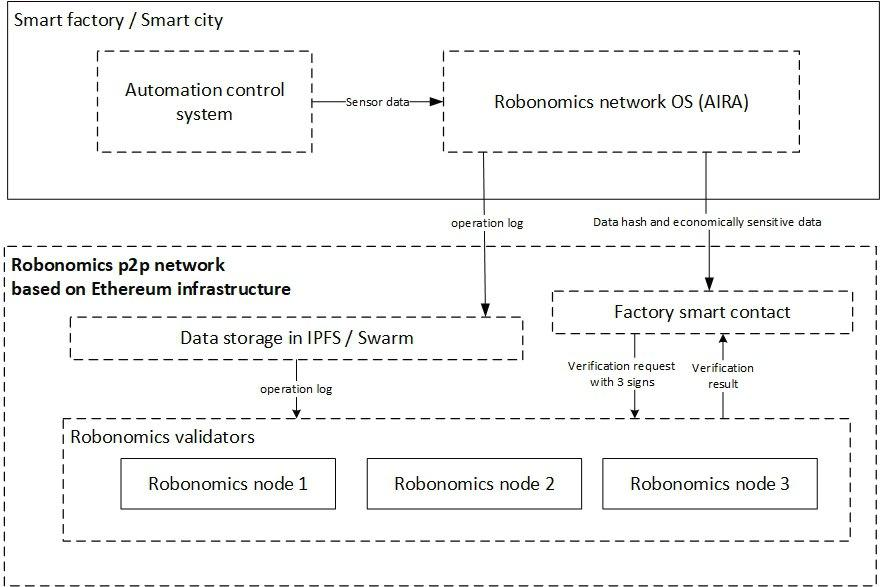
\includegraphics[width=1\textwidth]{app-3.png} 

Robonomics is able to monitor the performance of robots' contract liabilities by using models of verification the result of the machine's work. To do this, it is necessary that the contract liability indicates the desired observing network and the verification model.

The behavior model in accordance with the framework used by the engineer and robot is the main element of the work performance.

\subsubsection{The work algorithm of the observer's contract}

The contract initialization takes place in the same way as that of the lighthouse's contract; the participants deposit security to the contract, in proportion to which the quotas for verification of liabilities are issued.
\begin{enumerate}
	\item In the results channel, a message appears with the result for the liability requiring confirmation by the validator.
	\item The participant of the observing network uses a marker to sign the message with the result, and by its' decision sends it to the results channel.
	\item The lighthouse catches the message with validator's confirmation, but it cannot be located in N blocks.
	\item If the other participants in the observing network do not agree with the current owner of the marker, they can publish the messages with their decisions to the results channel.
	\item If the BFT is reached according to a decision that was not discussed with the current owner of the marker, then this transaction can be immediately placed in liability contract, and the current owner of the marker loses the quota.
	\item The commission in XRT is transferred to the participant in the observing network for the verification of the contract liability.
\end{enumerate}

\section{Robonomics Token, XRT}

The task of the Robonomics token is to ensure the operation of a decentralized network for the maintenance of Smart Cities and Industry 4.0 in the Ethereum infrastructure. In order to achieve this goal, the token economy needs to reflect the incentives for the implementation of the network's useful function by independent providers. These incentives should be distributed between the emission and the commission in such a way as to ensure the capacity of Robonomics in Ethereum—depending on the price of XRT token—as well as to motivate providers to run the Robonomics program in EVM with the data offered by users.

\subsection{Emission for execution of the Robonomics program in the Ethereum computer}

There is an interesting feature of emission in Bitcoin and Ethereum: regardless of whether or not there are transactions, the blocks are still created. This relative "indifference" allows the network to guarantee its capacity in accordance with the communication protocol. Emission is the key incentive for miners to maintain a given throughput, without waiting for the accumulation of a profitable total commission in the block.
 
Representing Robonomics as a program for EVM allows us to connect the emission of XRT tokens with the amount of recycled gas as a metric that is common for evaluating the calculation and saving of data of any program in the Ethereum computer. This will ensure the dependence of the Robonomics capacity in the overall Ethereum infrastructure from the price of an XRT token.
 
Let us introduce the basic technical unit of Robonomics called Wiener (1 XRT = 109 Wn) and define the following function of it:
\\
\\
\textit{Emission of 1 Wn = 1 gas utilized by Robonomics}
\\
\\
Such model stipulates:
\begin{enumerate}
	\item 1 XRT is not equal to 1 ETH because 1 gas may cost different amount of wei.
	\item The cost of 1 Wn must cover the costs of the provider for the disposal of 1 unit of gas in Ethereum.
	\item Only the Robonomics program should be able to perform Wn emission.
	\item Any increase in XRT price will contribute to the increase of the Robonomics capacity.
	\item The total capitalization of XRT may be greater than the capitalization of ETH, since it has an additional function apart from the utilization of gas in EVM.
\end{enumerate}

In order to achieve the rate of emission of \textit{Emission of 1 Wn = 1 gas utilized by Robonomics}, we offer:
\begin{enumerate}
	\item During the TGE by means of the Dutch auction, find the initial Wn emission multiplier to cover the minimum necessary expenses of the providers to ensure the presence of Robonomics in the Ethereum infrastructure at the initial moment of the emission.
	\item Introduce the stage of network development, during which the emission multiplier will be algorithmically reduced depending on the total volume of the utilized gas in the execution of the Robonomics program in EVM.
	\item In the future, ensure a permanent Wn emission for each utilized unit of gas by Robonomics in Ethereum.
\end{enumerate}

\subsubsection{TGE and the Dutch auction}

At the initial moment of Robonomics launch, we propose to issue 10,000,000 XRT, out of which from 5\%to 77\% will be available for the Dutch auction. We set a goal of N ETH for a fundraiser which will be directed to the account of a specially created Robonomics Foundation, which will support the development of the basic concept of representing CPSs as economically autonomous agents. The more models of economically autonomous agents available for use appear in the world, the higher the likelihood of making Robonomics work in general.
 
As a result of the auction, all participants will receive tokens at the lowest possible price, and Robonomics will get the initial ratio of XRT to ETH. Combining these data with the current gas price statistics, we will be able to determine the initial emission multiplier for the period of the development of Robonomics in the Ethereum infrastructure in order to cover the costs of providers at a competitive price, given the naturally lower capitalization of Robonomics as compared to Ethereum at the initial stage. According to our calculations for the spring of 2018, the minimum competitive price in the Ethereum network is the price of 2 gwei per 1 gas.


\subsubsection{Development}

We divide the period of Robonomics development in the Ethereum infrastructure into 5 epochs, each of which is statistically estimated in the total volume of the utilized gas in Ethereum. At its' conclusion, the epoch algorithmically reduces the emission multiplier in such a way that, at the end of the development period, the following condition is fulfilled:
\\
\\
\textit{Emission of 1 wn = 1 gas utilized by Robonomics}
\\
\\
That is, the multiplier should drop to one, disappear in the past.
\\
\\
Below is a table of the parameters of the five epochs of Robonomics development:
\\
\\
\begin{tabular}{ |l |l |l |l}
 \textbf{Epoch} & \textbf{Utilized gas} & \textbf{E(i), Wn} & \textbf{E(i), XRT} \\ 
 \hline
 1 &  3,47E+12 & 2,08E+13 & 2,08E+06 \\ 
 2 &  3,47E+12 & 1,39E+13 & 1,39E+06 \\ 
 3 &  3,47E+12 & 9,26E+12 & 9,26E+05 \\ 
 4 &  3,47E+12 & 6,17E+12 & 6,17E+05 \\ 
 5 &  3,47E+12 & 4,12E+12 & 4,12E+05 \\ 
 Total &  1,74E+13 & 5,43E+13 & 5,43E+06 \\ 
\end{tabular}

We allow for the volume of gas in the block as a constant value, since it is virtually impossible to predict its' growth for today. Accordingly, we can only judge that the transit of each epoch means the utilization of the percentage of gas according to the data on the size of the block in Ethereum for the period of spring 2018. At the end of the fifth epoch, we can say that Robonomics has reached the indicator of one annual volume of gas that was available on the Ethereum network in spring 2018. In any case, these statistics will be sufficient for an objective assessment of Robonomics growth in reference to the moment of TGE in 2018.

\subsubsection{Further emission}

After passing the development stage, Robonomics will reach a constant amount of emission quantitatively equal to the desired indicator Emission of 1 Wn = 1 gas utilized by Robonomics.

This linear relation will contribute to ensuring the minimum capacity that providers can ensure after equalizing the capitalization of Robonomics without a commission.

\subsection{Commission for launching the Robonomics program in the Ethereum infrastructure}

The first difference between the implementation of the Robonomics program with actual participants in EVM from the simulation is an indefinite period of time from the moment of creating the contractual obligation for the CPS, to the moment of sending the work product and finalizing the program execution based on this transaction. This implies that the CPS should be interested in paying the commission to the network, covering the provider's expenses for work in the communication channels to find the CPS with coordinated supply and demand, as well as the costs of settling the transaction to create a contractual obligation in the Ethereum Blockchain.

\subsection{XRT token's additional tasks}
\subsubsection{User commission enables observing networks existence}

There is no need to motivate providers to finalize the implementation of the Robonomics program, taking into account the observing network or not. Any provider will happily finalize the implementation of the Robonomics program for the sake of the emission.
 
Therefore, the CPS service user's commission can only be used to pay for the verification of the results of the CPS behavioral model execution.

\subsubsection{XRT accumulated on the lighthouses' accounts as the trust mechanism of Robonomics}

At the zero time of Robonomics existence, providers will be interested in creating "individual" lighthouses with a minimum rate of XRT for the contract of the lighthouse, in the format of security. Once supply and demand emerge in Robonomics, the interest in working on a particular lighthouse will be higher, and the total commission that the provider can receive from the communication channel served by this particular lighthouse will be larger. Over time, providers will begin to consolidate around those lighthouses where the share of the provider's security placed on the lighthouse contract will give enough time to get additional benefits.
 
Ultimately, the higher the total commission from certain communication channels, the larger the XRT share that providers will be ready to freeze. The larger the amount of frozen funds at a certain lighthouse, the higher other participants' trust in this lighthouse's operation and Robonomics in general.

\subsubsection{XRT as the quantitative reflection of network's capital}

The Robonomics' capital is nothing more than a reflection of the value of the network using the Ethereum infrastructure to build up communications with economically autonomous CPSs.
 
Capital growth of such a network will represent the growth of the number of people in the society who accept the idea of CPSs as autonomous economic agents. On the other hand, Ethereum will be viewed as an infrastructure suitable for economically meaningful communication based on academic and industrial automation standards.

\subsubsection{Cybernetics market}

In the long term, XRT will turn into the internal currency of the market for contractual robot to robot liabilities, being initially the token necessary for CPS to enter into contractual obligations and verify their result. That will be the market in which each program execution will be looped into program execution.

\subsubsection{Conclusions about the movement of XRT in Robonomics network}

To conclude, here is what we have: XRT emission is designed to maintain the constant readiness of Robonomics to execute the communication with the CPS as an autonomous economic agent in the Ethereum infrastructure. Commissions create an incentive for the use of user data in the execution of the Robonomics program by providers.

\subsubsection{Denomination }
\begin{tabular}{ l |l |l |l |l}
 Value &  $1$ & $10^3$ & $10^6$  & $10^9$ \\ 
 \hline
 Title in the Robonomics platform &  wiener & coase  & glushkov & robonomics token\\ 
\end{tabular}

\section{Description of Robonomics work}
\subsection{Proposal of a new behavioral model by an engineer}

\begin{wrapfigure}{l}{0.30\textwidth} %this figure will be at the right
    \centering
    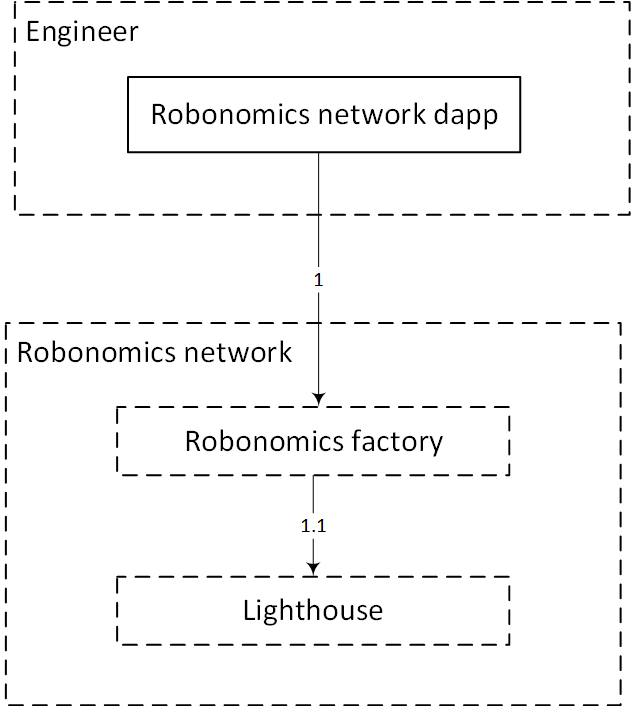
\includegraphics[width=0.30\textwidth]{step-by-step-1.png}
\end{wrapfigure}

A lighthouse in an autonomous workflow, allowing the distribution of providers' work time and serving a particular broadcast channel.

Robonomics factory is an autonomous workflow allowing the creation of a new lighthouse or liability contract using the appropriate libraries stored on the Ethereum Blockchain.

Organizations that create cyber physical systems may be interested in presenting their robots as services that can manage their own economies: from obtaining technical and financial parameters before rendering the service, to independently providing their work with the necessary resources and services using the funds that CPS controls.

To fulfill such tasks, the engineer can create a ROS-compatible behavioral model that he wants to propose to cyber-physical systems' owners in order for their robots to start working as an economically autonomous system.

The engineer uses dapp to connect to the Robonomics network and sends a transaction (1) to Ethereum containing a hash of the ROS-compatible cyber physical system's behavioral model.

Based on the transaction from the engineer (1), there is an internal call (1.1) to create a new autonomous Lighthouse workflow in the Ethereum Blockchain.

\subsection{Start of work of the Robonomics network provider}

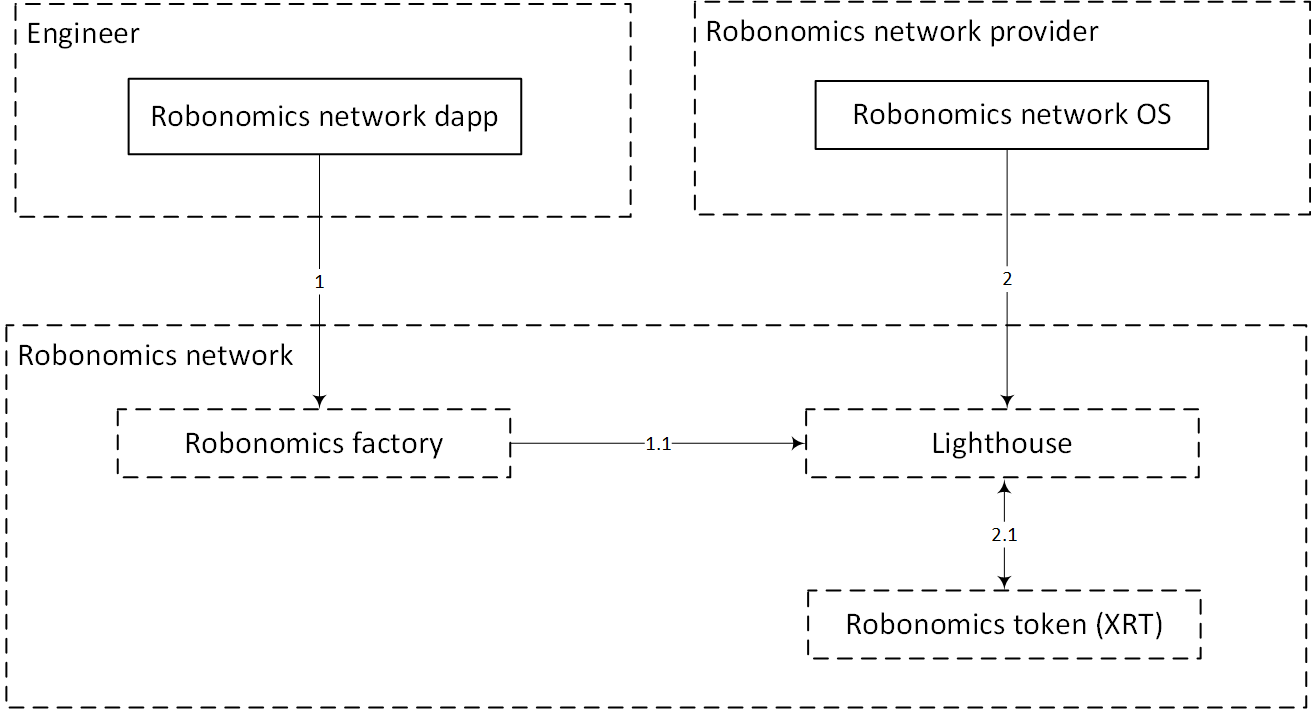
\includegraphics[width=1\textwidth]{step-by-step-2.png}

The Robonomics network provider sends transaction (2) to the created (1) Lighthouse, transferring a number of XRT tokens (2.1) as the allowance used in the distribution of the lighthouse working time among the providers.

\subsection{Start of the cyber physical system work as a service}

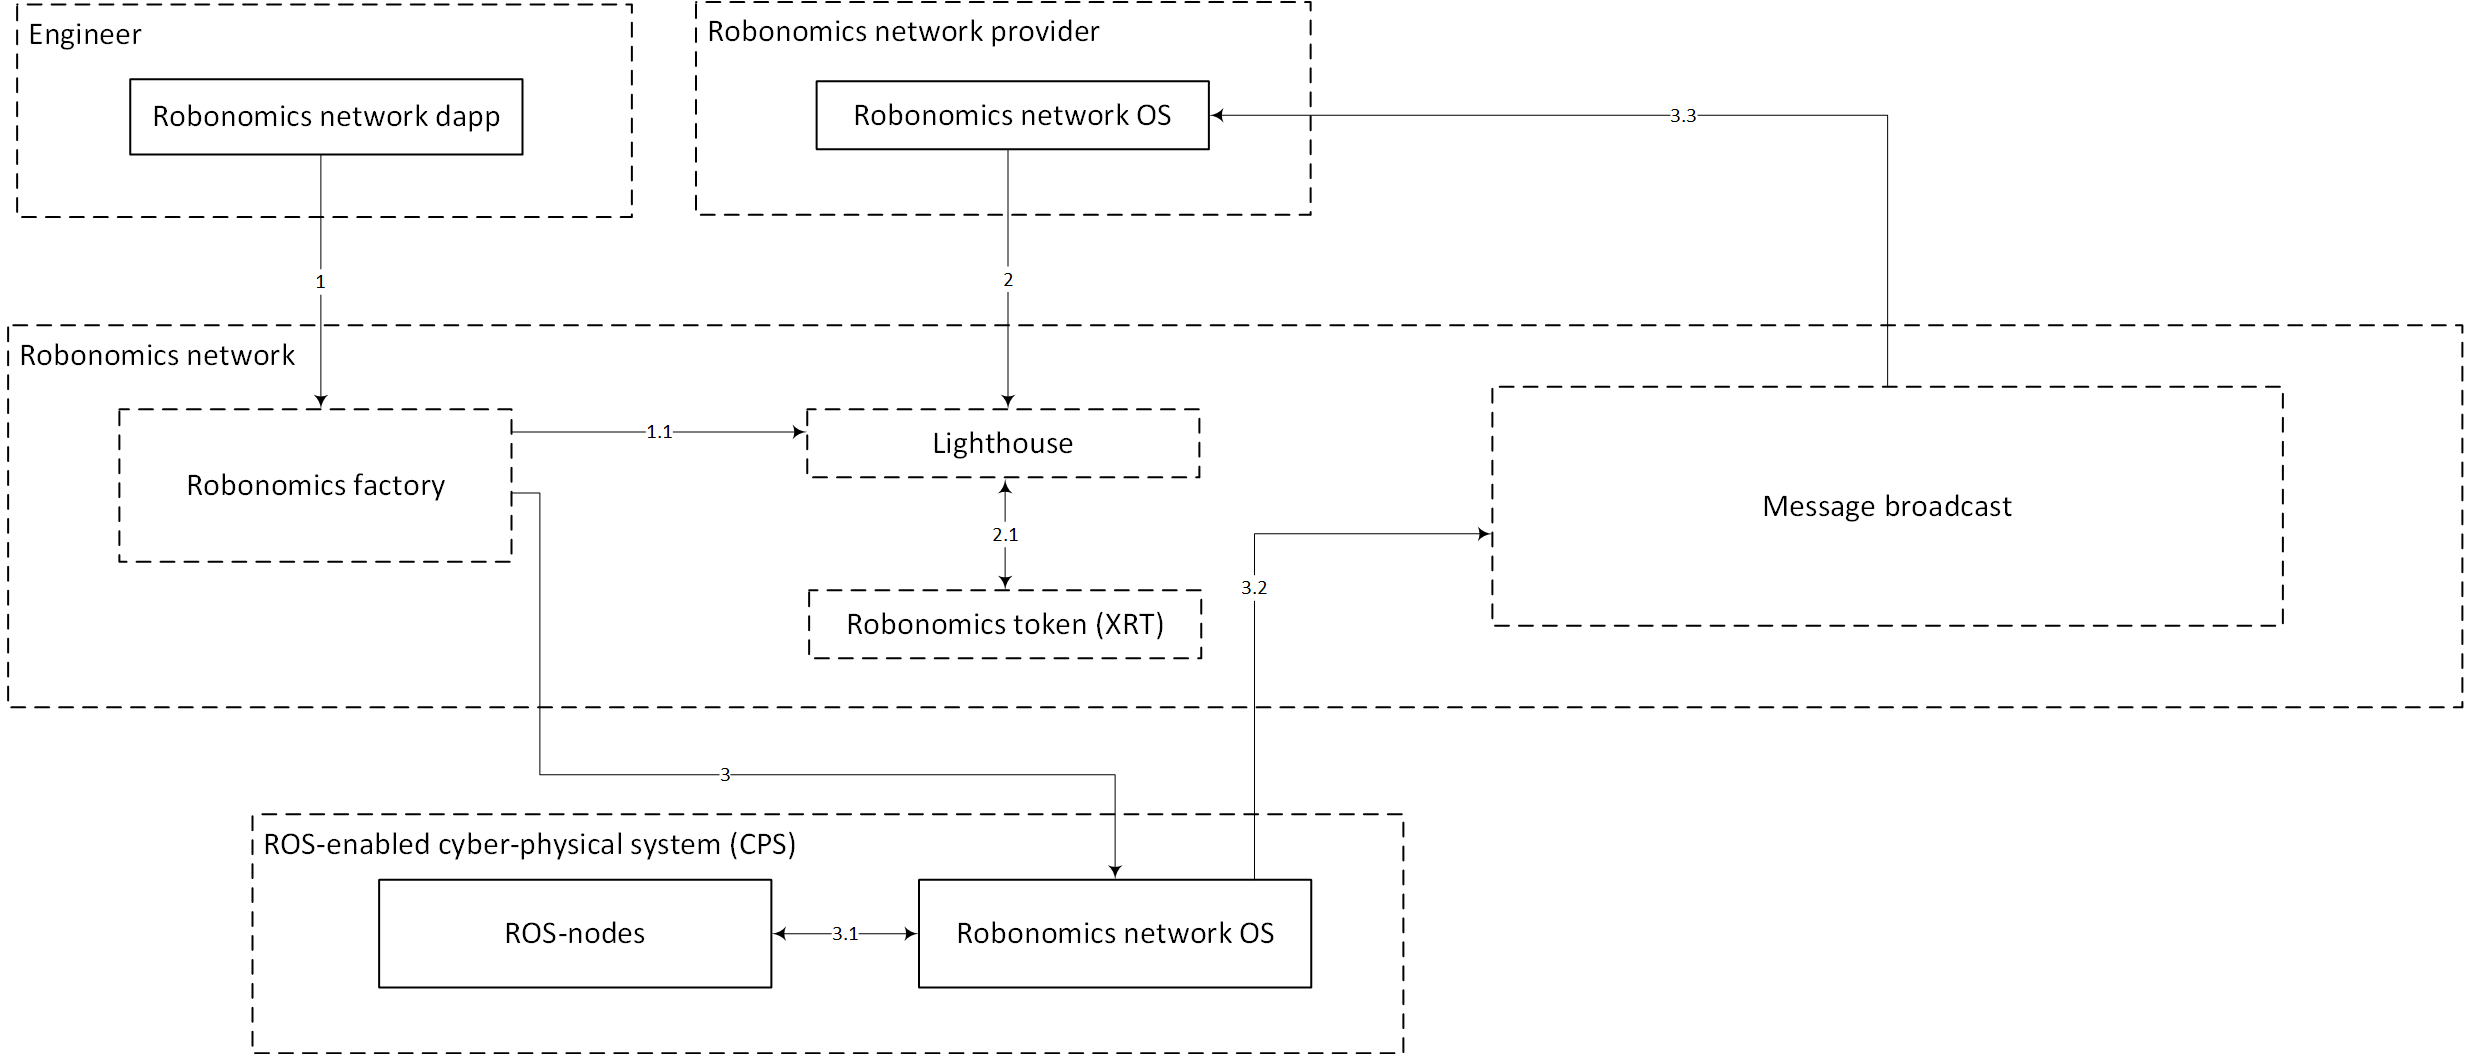
\includegraphics[width=1\textwidth]{step-by-step-3.png}

Robonomics network OS receives a list of created lighthouses from the Robonomics factory (3). Using the information from the description of lighthouses and addressing its nodes (3.1), the CPS begins to publish its proposals for providing services to the Robonomics broadcast channels (3.2).

The Robonomics network provider receives a message through the broadcast channel that a new offer by the CPS was published (3.3).

\subsection{The appearance of the user in the Robonomics network}

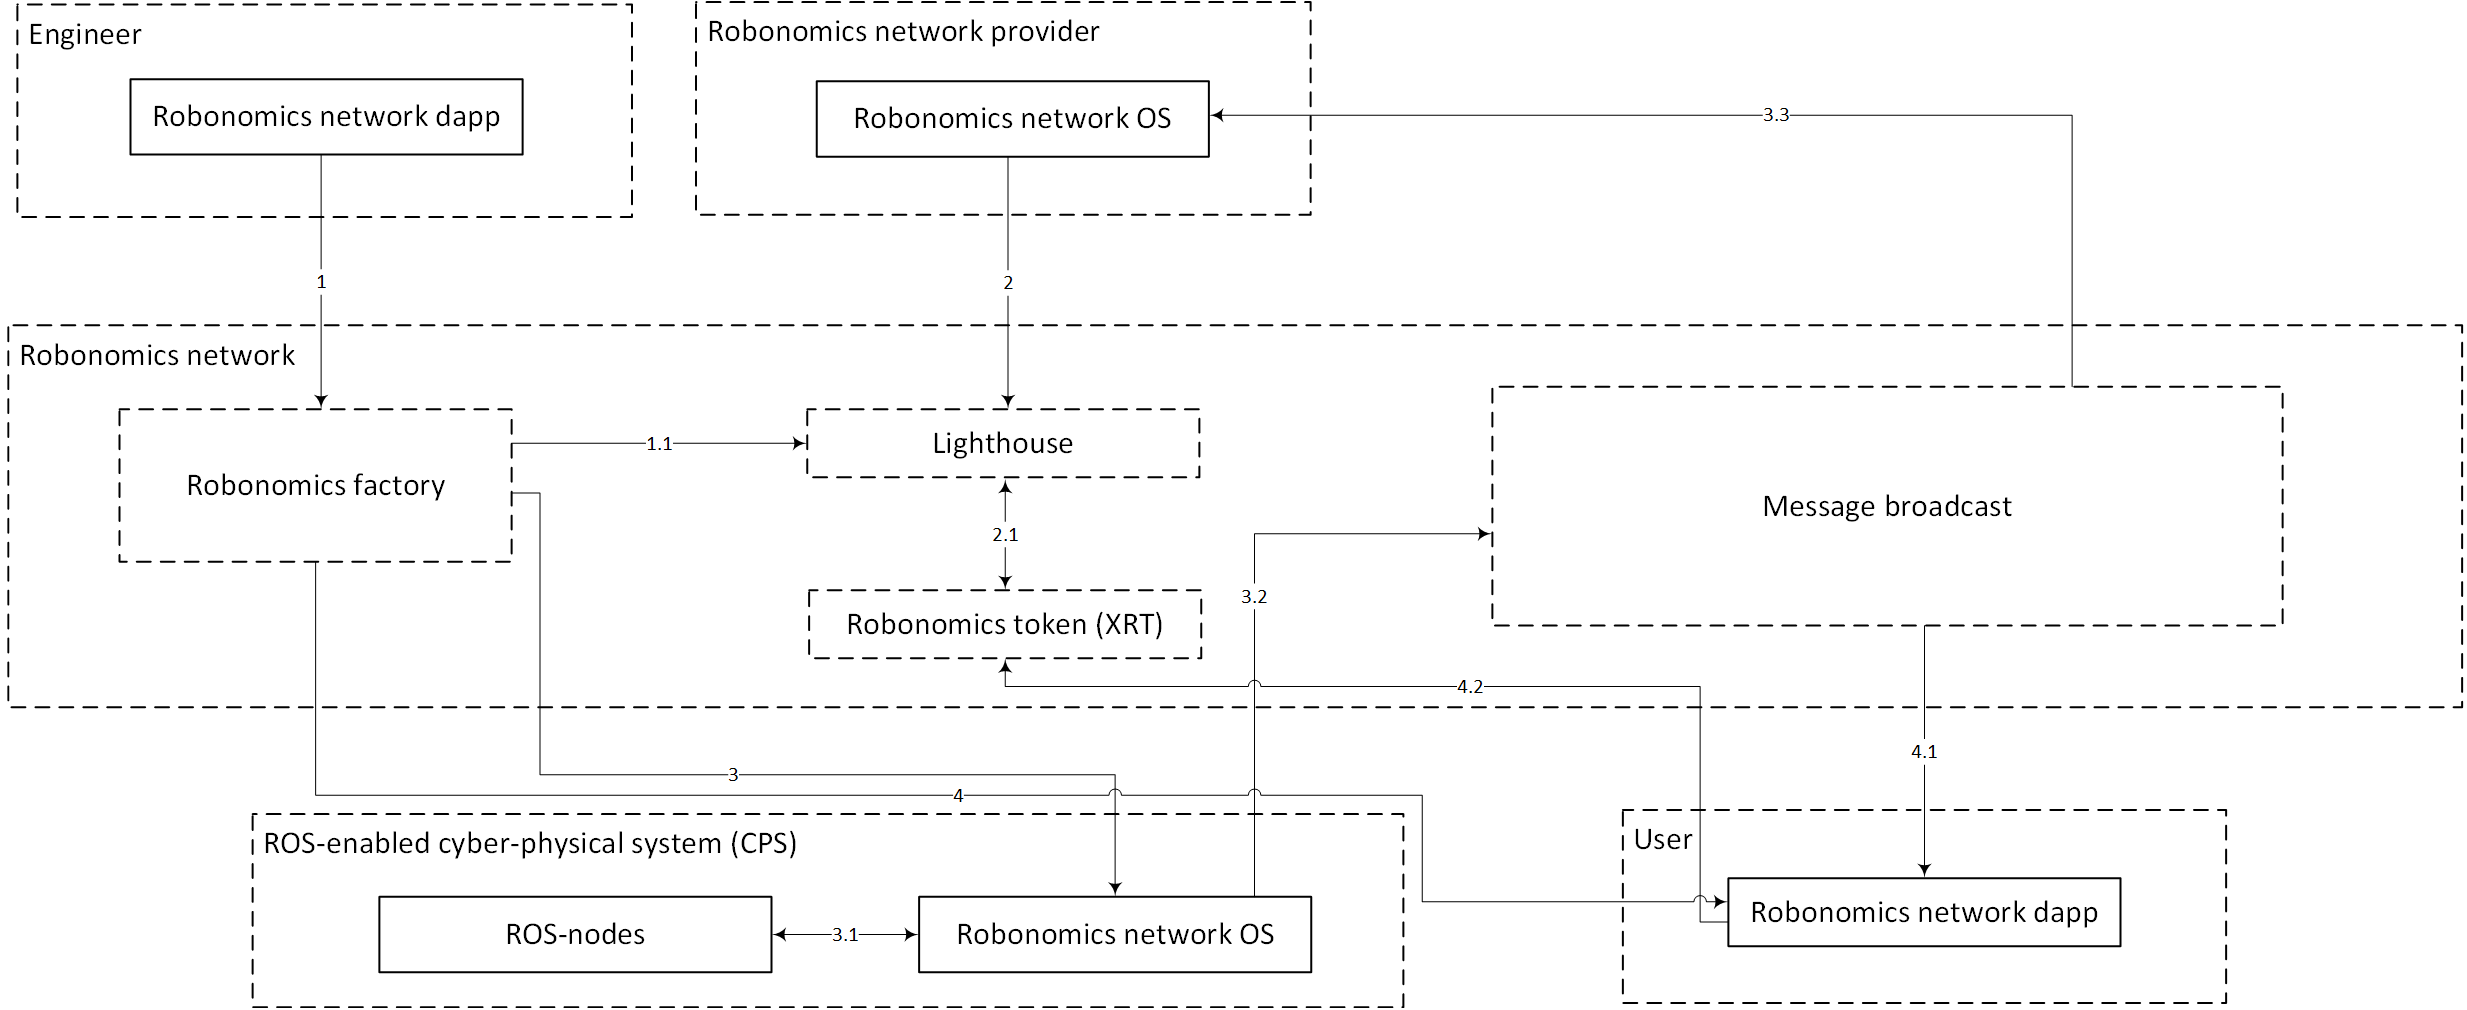
\includegraphics[width=1\textwidth]{step-by-step-4.png} 

The user receives a list of the Robonomics broadcast channels (4) with the help of dapp and starts listening to the messages in these channels (4.1). The user, making sure that there is a service by the CPS (3.2) he is interested in in the Robonomics network, sends a transaction to the Ethereum Blockchain in order to allow the withdrawal of XRT tokens by the autonomous working process of the Robonomics factory (4.2).

\subsection{Creation of the liability to perform a service by the cyber physical system}

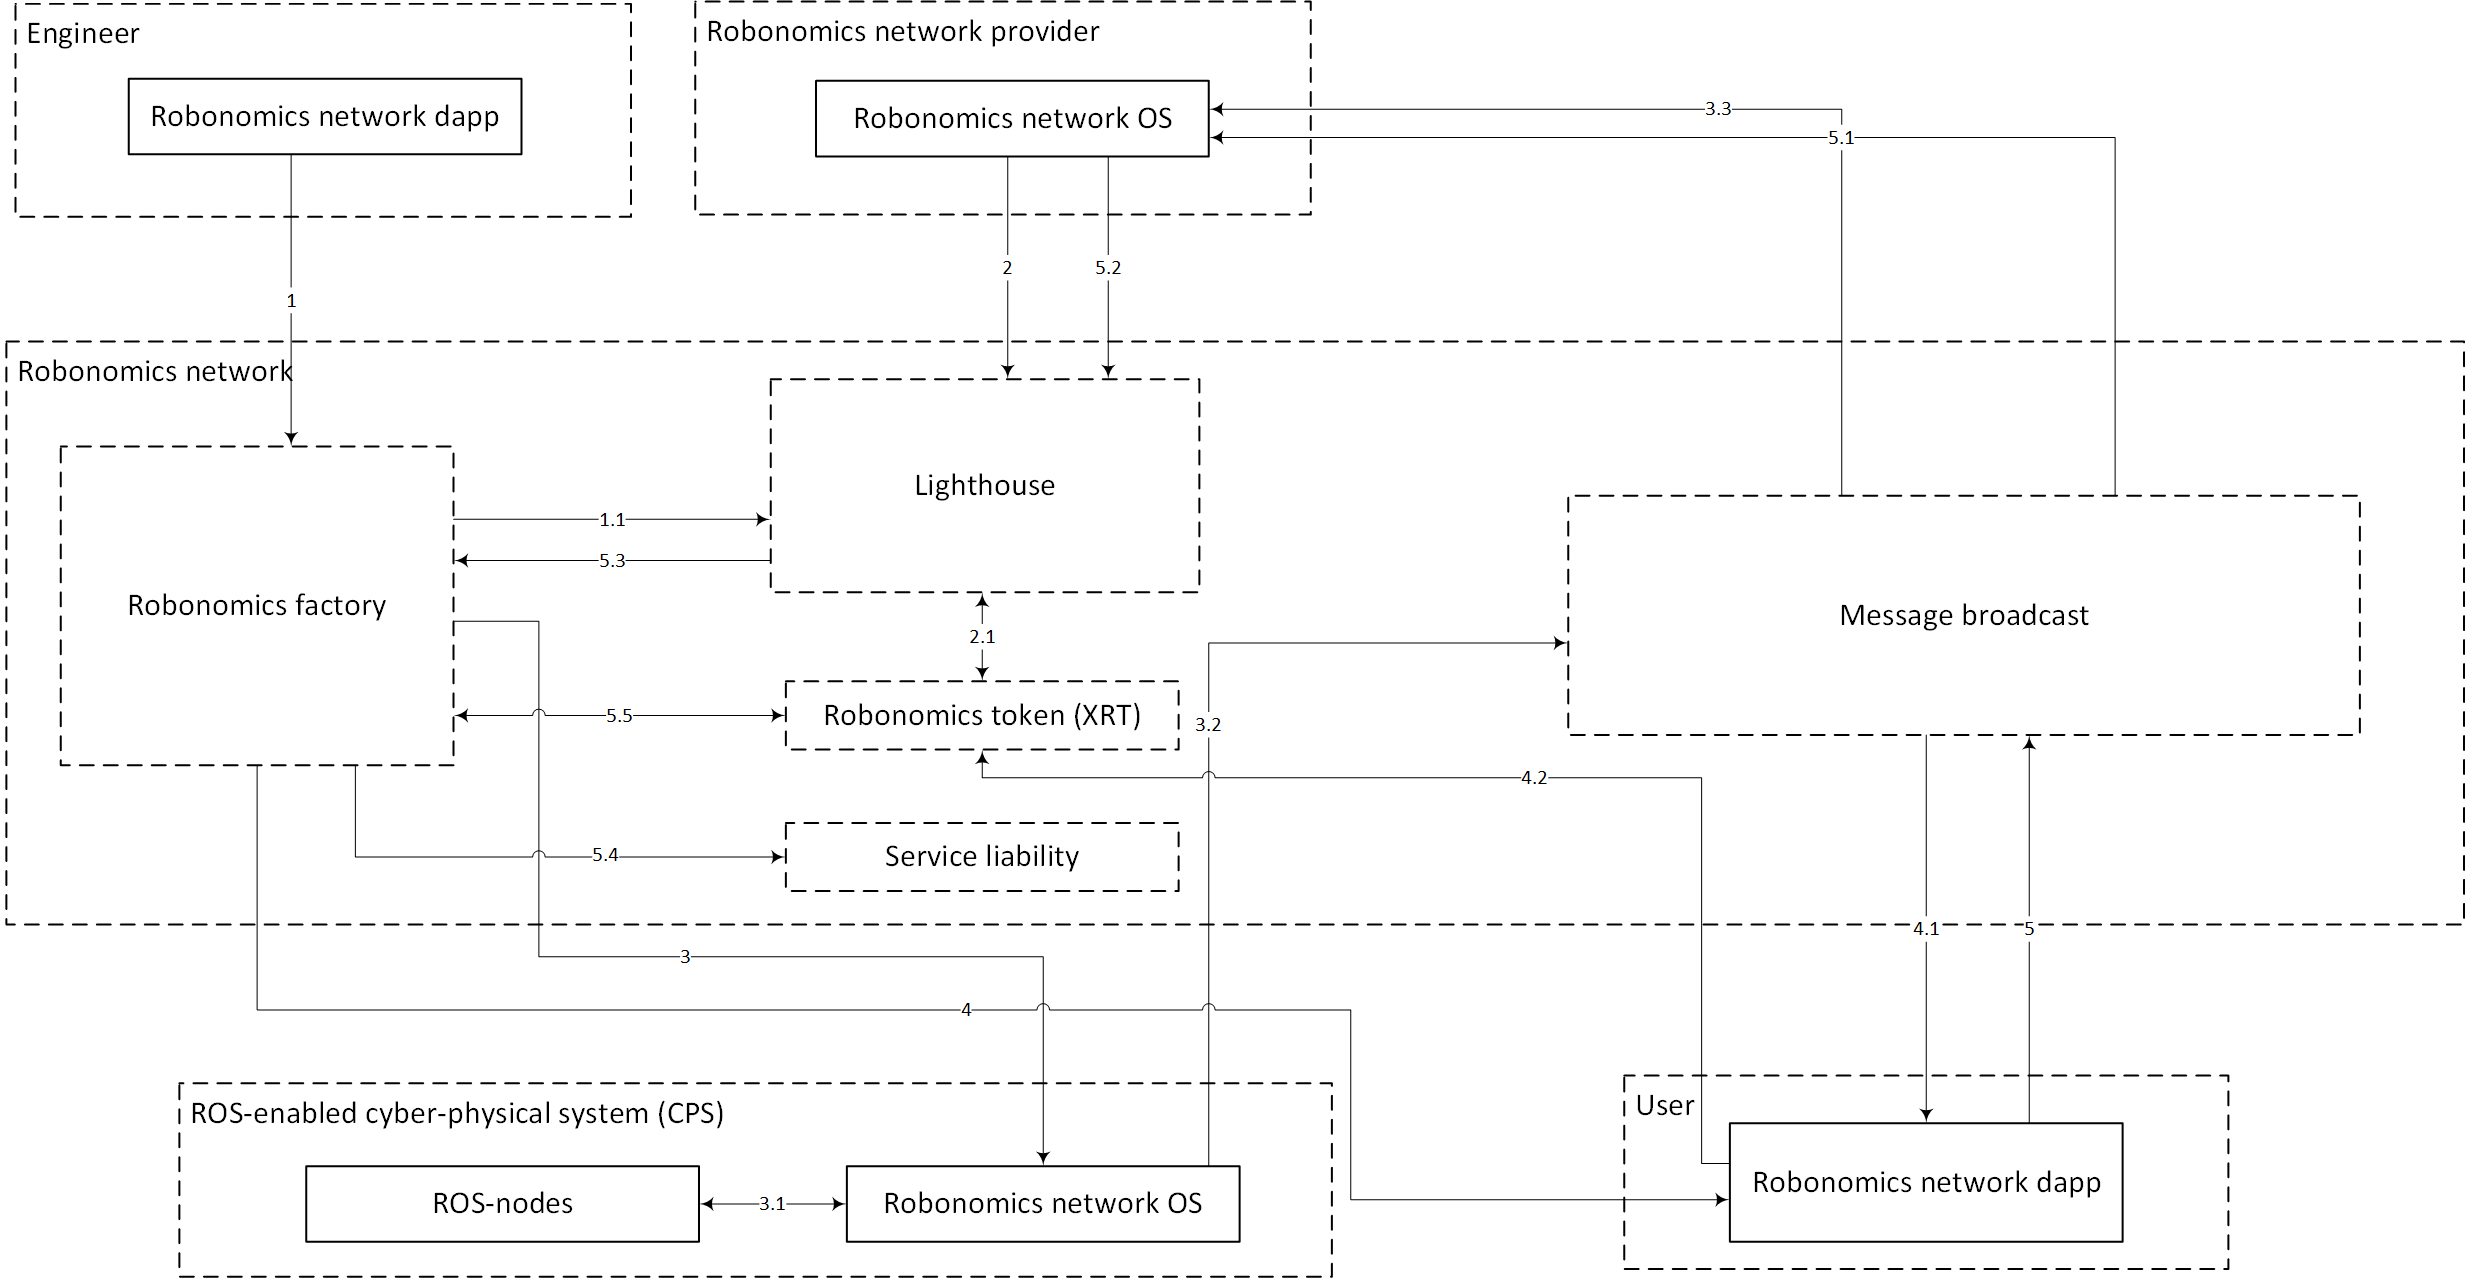
\includegraphics[width=1\textwidth]{step-by-step-5.png} 

The user, having enough XRT tokens to place demand for the service of his interest, can send a message about his demand (5) to the previously published CPS service (4.2) in the broadcast.

The Robonomics network provider having received the user's message (5.1) and maintaining a locally stored message from the CPS (3.3) that are matched by the hash value from the behavioral model of the ROS-compatible CPS and the cost of the service rendered, refers to the Lighthouse's autonomous workflow (5.2) transmitting deferred signatures of both parties.

The lighthouse addresses the Robonomics factory (5.3) in order to create a liability for rendering a service (5.4), the factory, by creating a liability contract and knowing its address on the Ethereum Blockchain, addresses the XRT contract  (5.5) for:
\begin{enumerate}
	\item Transfer of the service cost from the user's account (4.2) to the contract's account;
	\item Emission of XRT tokens to the contract's account, namely the total amount required to utilize the gas multiplied by the starting factor on the Ethereum Blockchain.
\end{enumerate}

\subsection{Liability execution by the cyber physical system}

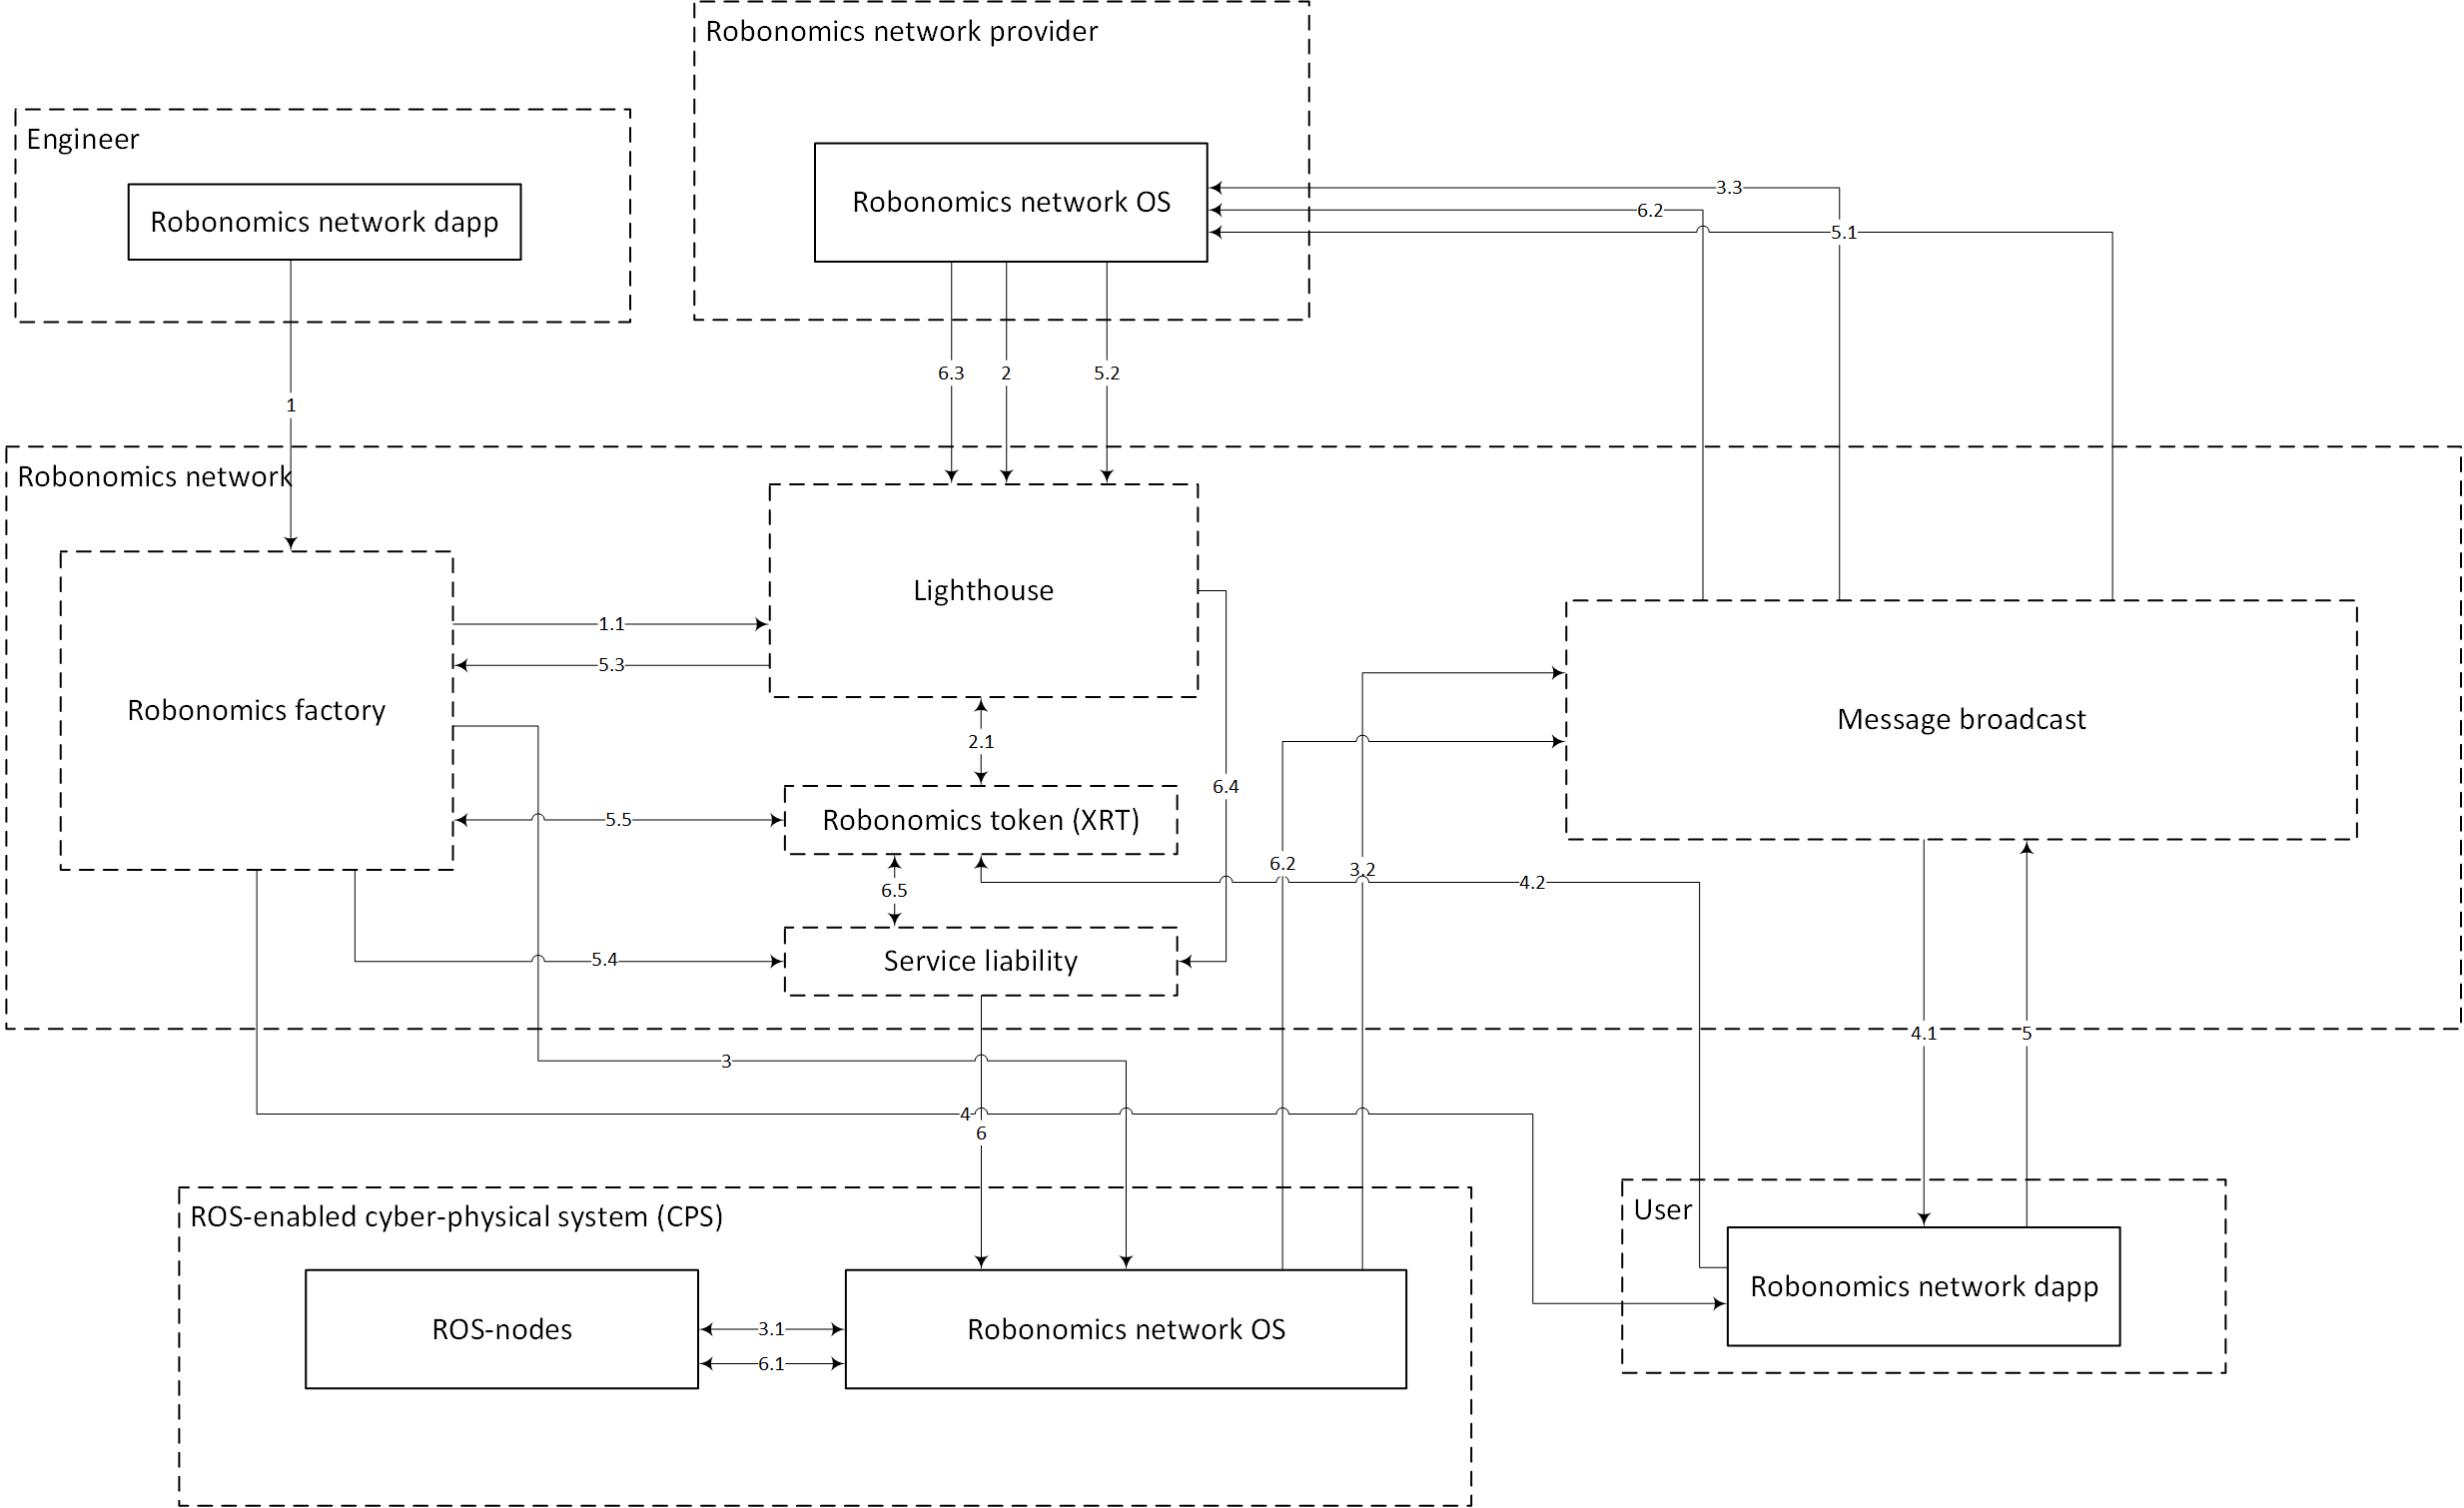
\includegraphics[width=1\textwidth]{step-by-step-6.png} 

The cyber physical system receives a notification about a liability contract created for it with the help of Robonomics network OS, in which it is possible to find out the hash of the behavioral model and the hash of the parameters (variables) of the behavioral model (6).

Having uploaded the behavioral model and parameters (6.1) for execution, the CPS with the help of ROS-bag starts executing the received liability.

During execution, the CPS forms an operations log and after the completion of work sends its hash to the Robonomics communication channel serving this behavioral model (6.2).

The Robonics network provider receives the hash of the log (6.2) and sends a transaction about the fulfillment of the liability by the CPS (6.3) in the Ethereum Blockchain to the Lighthouse (6.3). The Lighthouse creates an internal transaction to the corresponding service liability and locates the hash of the CPS operations log (6.4) there. The liability contract then releases the fee for the rendered service to the CPS address, as well as emits XRT to the address of the provider who sent the transaction to the Lighthouse.

\section{Robonomics platform applications}

\subsection{Building trust to the production of smart cities and smart factories}

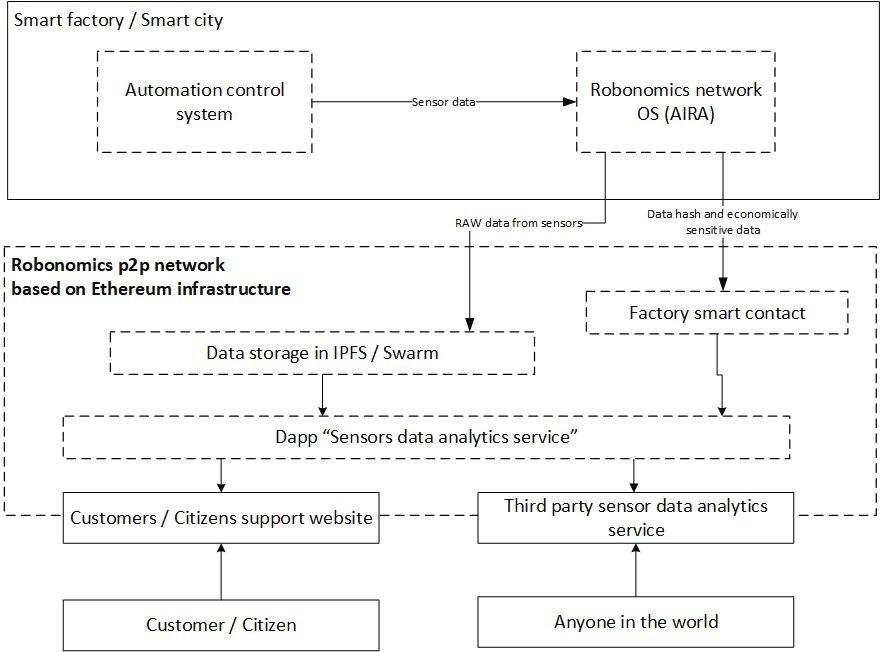
\includegraphics[width=1\textwidth]{app-1.png} 

The trust issue between the consumer and the smart factory lies in how the consumer can be sure of the quality of the product produced by the smart factory. The products in the store can be similar, but have a very different story of origin. We propose to record the technological process, placing it in a decentralized network. Hash from the log of CPS operations is saved in the blockchain, giving the history of the product the property of immunity. The consumer is confident in the product, since its' history cannot be changed in the future.

\url{https://github.com/airalab/robonomics_comm/blob/master/robonomics_liability/src/robonomics_liability/executor.py#L50}

Here the data of the production process is collected and accumulated at the time the liability is being fulfilled by a smart factory.


\begin{lstlisting}
 {
	msg.result = self.ipfs.add(result_file)['Hash']
	self.complete.publish(msg)
  }
\end{lstlisting}


The operations log is stored in the IPFS network, and its hash is published in the contract liability and cannot be changed in the future.

\subsection{Smart factory launch by the user}

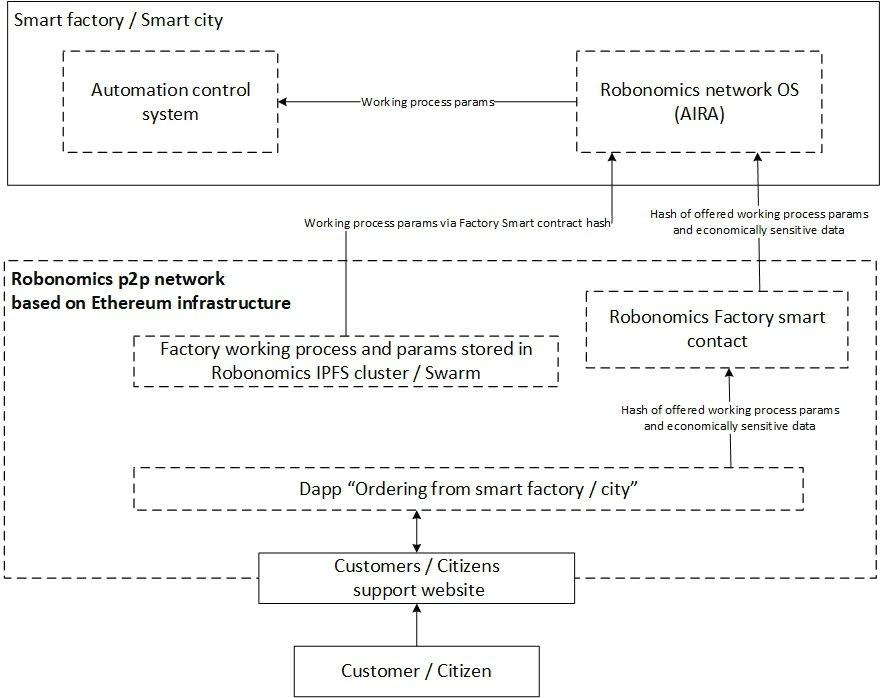
\includegraphics[width=1\textwidth]{app-2.png} 

The problem of accessing the factory as a service for the consumer lies in eliminating the intermediary that can somehow affect their interaction. In this regard a smart contract is a suitable object.

\url{https://github.com/airalab/robonomics_comm/blob/master/robonomics_liability/src/robonomics_liability/executor.py#L34}

Here the smart factory follows the events from the factory of smart contracts, accepting liabilities in which it is listed as the executor.

\begin{lstlisting}
rospy.logdebug('Getting objective %s...', msg.objective)
self.ipfs.get(msg.objective)

player = Player(msg.objective)
player.start()
\end{lstlisting}

Once the liability is undertaken, the smart factory begins its execution by downloading the liability parameters from the IPFS and reproducing their sequence locally.

\subsection{Managing the economy of robots with the help of capital}

Let us imagine a set of economically independent cyber physical systems or just robots as a vector (R), and capital (investment) as a vector (K). Here vector $ R = {R_i, i=\overline{1,n}}$, where $R_i$ — number of robots at the market i, n — the number of examined markets. And vector $ K = {K_j, j=\overline{1,n}} $, where  $K_j$ — investments to the j-th market. Let us describe the model of robots distribution in the market proportional to the capital as follows: 
\[
R'[k] = K[k] * { \sum R_i[k] \over \sum K_i[k] }
\]
\[
e[k] = R'[k] - R[k-1] ;
\]
Here:
\begin{itemize}
\item $R'[k]$ — desired distribution of robots in the markets [number];
\item $R[k-1]$ — the number of robots already present at this capital's market;
\item e — vector of distribution errors (deviation from the desired value of distribution) [number];
\item $i \in \overline{1,n}$ - market index;
\item k - discrete time step;
\item $\sum R_i[k] $ - the number of robots in all the markets in question at step k;
\item $\sum K_i[k] $ - the amount of investment in the markets in question at step k.
\end{itemize}

Based on the described above, we can formulate the law of managing the economy of robots as follows:

Every robot should strive to participate in the market where the distribution error is higher \cite{LonshakovSergey2017HowProtocol}.

When the next robot is included in the economy, the market for placing its offer by this robot is chosen from the equation:

$ i = maxi(e[k])$, which leads to $ e_i[k] \rightarrow 0 $.

Here  $ maxi(e) $ - index of the maximum element of the deviation vector.

\subsubsection{Reference implementation}

The implementation of the Robonomics management algorithm is contained in the package robonomics\_control

\url{https://github.com/airalab/robonomics_comm/tree/master/robonomics_control}. 

Here the linear distribution algorithm is based on the information from the smart contract on the distribution of capital and information from markets about the lots received from cyber physical systems.

\url{https://github.com/airalab/robonomics_comm/blob/master/robonomics_control/src/robonomics_control/distribution.py}

\subsection{Tokenized values based on the robot's labour}

Consider the scenario for the release of carbon units by a sensor in a smart city. The sensor is empowered to emit a token of carbon units if the air pollution is below a certain value.

Let the sensor as a result of the liability measure the degree of air pollution send the number of carbon units released, together with the results. We extend the standard liability contract by a method that takes the number of units for emission together with the result of work.
\begin{lstlisting}
function setResult(bytes32 _result, uint256 _emission);
\end{lstlisting}


This way, the values for the release of carbon units are retained in the liability contract. Provided that the network of observers confirms that the sensor's measurements are correct, a corresponding number of tokens will be emitted according to the liability contract.

\begin{lstlisting}
function confirm() {
  ... 
  carbonToken.emission(emission);
}
\end{lstlisting}

It is important that the liability contract is added to the group that has access to the token's emission, which the factory made at the inception stage. The factory of liability contracts is then obliged to possess the information on conformity of the set behavioral model to such token, which can be emitted upon the successful performance of the liability.

\section{Scalability}

Robonomics is designed to represent such large cyber physical systems as, for example, a whole factory or city. The current capacity of the Ethereum network is sufficient to enforce over 1,000 contractual obligations per day. This is enough for:
the organization of daily direct order by car buyers on the sites of several auto groups such as BMW, Porsche and Avtovaz.
Registration of regular routes for unmanned logistics of the current global industrial zones.
Daily publication of reports on the state of the environment from sensory networks of all cities in the world with a population of over 1,000,000 people.

\section{Robonomics segment in Ethereum}

With the introduction of the ability to create your own segment in the Ethereum network, Robonomics can form a segment with an increased capacity, and also allow multiple rises in the number of possible contractual performances by robots. This serves to cover the request of the entire Industry 4.0 with transaction costs over 1,000 \$.

\section{Conclusion}

The Robonomics platform aims to solve the social and economic tasks of total robotization of mass production, city life and logistics. The main application of the platform is related to the tasks associated with building trust in the services and products of smart cities and factories, providing direct user access to autonomous cyber physical systems and managing multi-agent systems with the help of capital.

The Robonics platform will expand the capabilities of the Ethereum network infrastructure for use in such areas as Industry 4.0, IoT and smart cities.
\newpage
\printbibliography
\newpage
\section*{Appendix 1: Questions at the junction of robotics and economic theory}

Total robotization. The arrival of robots into the life of every person is inevitable. Machines are able to perform tasks inaccessible to a man, they are more effective in many types of operating activities and save people time in their daily routines already today.

The development of robotics has reached a stage where problems of communication between physically or logically separated autonomous agents-robots having the right to decide what actions are appropriate as part of their existence have appeared. Technologies used in the world of machines expand the range of solutions available to the robot, which increases its level of autonomy each time.   

The communication tasks of autonomous robots are most clearly revealed in such ideas as Industry 4.0 and Internet of things. Below is the list of the most significant issues of autonomous robots' participation in human life, according to the authors of this work:

\begin{itemize}
	\item How to build trust to the production of the robotized services?
	\item How to ensure the ownership transfer to the consumer, if the process of production and logistics does not involve humans?  
	\item How does a fully automated enterprise outside the window understand the changing needs of a human?
	\item How to ensure direct interaction between robots of two different corporations?
	\item How to impose taxes upon robots' activities and what should be considered a separate robotized unit?
\end{itemize}

Different variants of answers to these questions entail various risks of increasing instability and the possible collapse of the world system - this is a challenge in building a society where there is no place for slave human labor.

\section*{Appendix 2: AIRA distribution}

The anchor (reference) implementation of the Robonomics OS is AIRA project (https://github.com/airalab/aira). AIRA distribution in based on NixOS GNU/Linux distribution and is being developed by an open community, of which Airalab developers are a part of.

\paragraph{NixOS}

The branch from the package database nixpkgs is the basis of the distribution (\url{https://github.com/airalab/airalab-channels}), where Airalab team added important Ethereum infrastructure packages (such as parity, web3.py); support of Robot Operating System, as well as fundamental packages of Robonomics communications stack: robonomics\_market, robonomics\_liability.

\paragraph*{ROS}

Minimal ROS support is provided within the ros\_comm metapackage with the use of the necessary basic stack of software for serialization and messaging between ROS network participants, calling services and integrating into a single rosgraph name space.
	
Based on the distribution, the installation images of the experimental factory stands are formed (\url{https://aira.life/cases/}): Game of trains, Industry 4.0 in use.

\section*{Appendix 3: External API AIRA}

\begin{tabular}{ l |l}
	/market/incoming/ask & Incoming messages with demand from the communication channel. \\
	/market/incoming/bid & Incoming messages with supply from the communication channel. \\
	/market/sending/ask & Outcoming messages with demand from the communication channel. \\
	/market/sending/bid & Outcoming messages with supply from the communication channel. \\
	/market/signing/ask & Outcoming messages with demand for signing. \\
	/market/signing/bid & Outcoming messages with supply for signing. \\
\end{tabular}

\section*{Appendix 4: DAO program}

\paragraph{Representation of the economy of robots as a program for the decentralized Ethereum computer}

In order to get a decentralized service, you need a decentralized computer and a program adapted to its specific character. Workflows that enable the use of the Ethereum network infrastructure for Smart Cities and Industry 4.0 can be presented as a program for the Ethereum computer.

Let us imagine that we have a program called "Robots Economy Network", we load it into the Ethereum Blockchain for storage. The program allows members of the Ethereum infrastructure to run the "Robots Economy Network" on their virtual machines and thereby organize a new service in a decentralized environment, acting as its provider.

\paragraph{Representation of the economy of robots as the DAO}

Autonomous workflows and their contractors form the DAO. The contractor can not influence the work of the DAO, he can only follow the instructions. Economic incentives should support the interest of the performer for the full implementation of the work process. The workflow can not be changed without consequences in the Ethereum Blockchain.

\end{document}
